\documentclass[a4paper,12pt,twoside]{article}
\usepackage{rhreport}

\title{River Mapping Report}
\author{immaculate.mwanja }
\date{July 2019}

\begin{document}

\maketitle

\newpage
\tableofcontents

\newpage
\section{Executive Summary}
\begin{multicols}{2}
HOT is an international NGO dedicated to humanitarian action and community development through open mapping. We work together to map data which revolutionises disaster management, reduces risks, and contributes to the achievement of the Sustainable Development Goals.
HOT develops open source apps and tools for collaborative mapping and geospatial data collection. Our tools are free for all to use and leveraged by partners such as Red Cross societies, Médecins Sans Frontières (MSF), UN agencies and programmes, government agencies, and local NGOs and communities.
OMDTZ.

\end{multicols}


\section{Introduction}

Several drone flights were to be  conducted along five major rivers of Dar es Salaam including  Msimbazi, Mpiji, Tegeta, Kizinga and Mzinga rivers, spanning 60 linear kilometers of waterways of Dar es Salaam’s critical water arteries. Msimbazi river was not mapped since it  was  already mapped by World bank. The drone flights provided a digital photographic mark-up of the current status of Dar es Salaam’s waterways.   
Drone flights enable studying any aggregations of waste/informal dumps that are on the banks of the waterways within fifty metres of its bank on either side.Such data is presented as three-dimensional imagery of waste aggregations, further assisting the study team to estimate rough waste volumes.

Drone flights consistently track and record spatial data relating to their own trips and correspond the GIS data with a set of other socio-political and economic indicators, to ease further analysis. This includes:   

\begin{itemize}
    \item The corresponding political division i.e. subward, ward and municipal boundaries—drone flight spatial data overlaid existing socio-political spatial data indicating, via simple desktop analysis, the political constituency that governs each spatial area the drone covers. This allows users to correspond with an informal/illegal dump with the relevant political office that governs the area.
    \item The corresponding density of the geography they are flown over i.e. buildings per sq km/population per sq km via census data. 
\end{itemize}

Drone flights for data collection were conducted within 44 calendar days from 5th April to 18th May 2019, contingent  to the Tanzania Civil Aviation Authority (TCAA) and Ministry of Defence permissions and suitable weather. All technical personnel and equipment required for this assignment are present in Dar es Salaam (site location). 

OMDTZ  combined drone flights and the existing spatial data to conduct a rapid desktop analysis of planned residential and commercial zoning and transport economics as they relate to solid waste management services.

\newpage
\section{Objectives}

\lipsum[0-1]


\begin{figure}%[H] % uncomment "[H] to force the image to the middle of the page
    \centering
    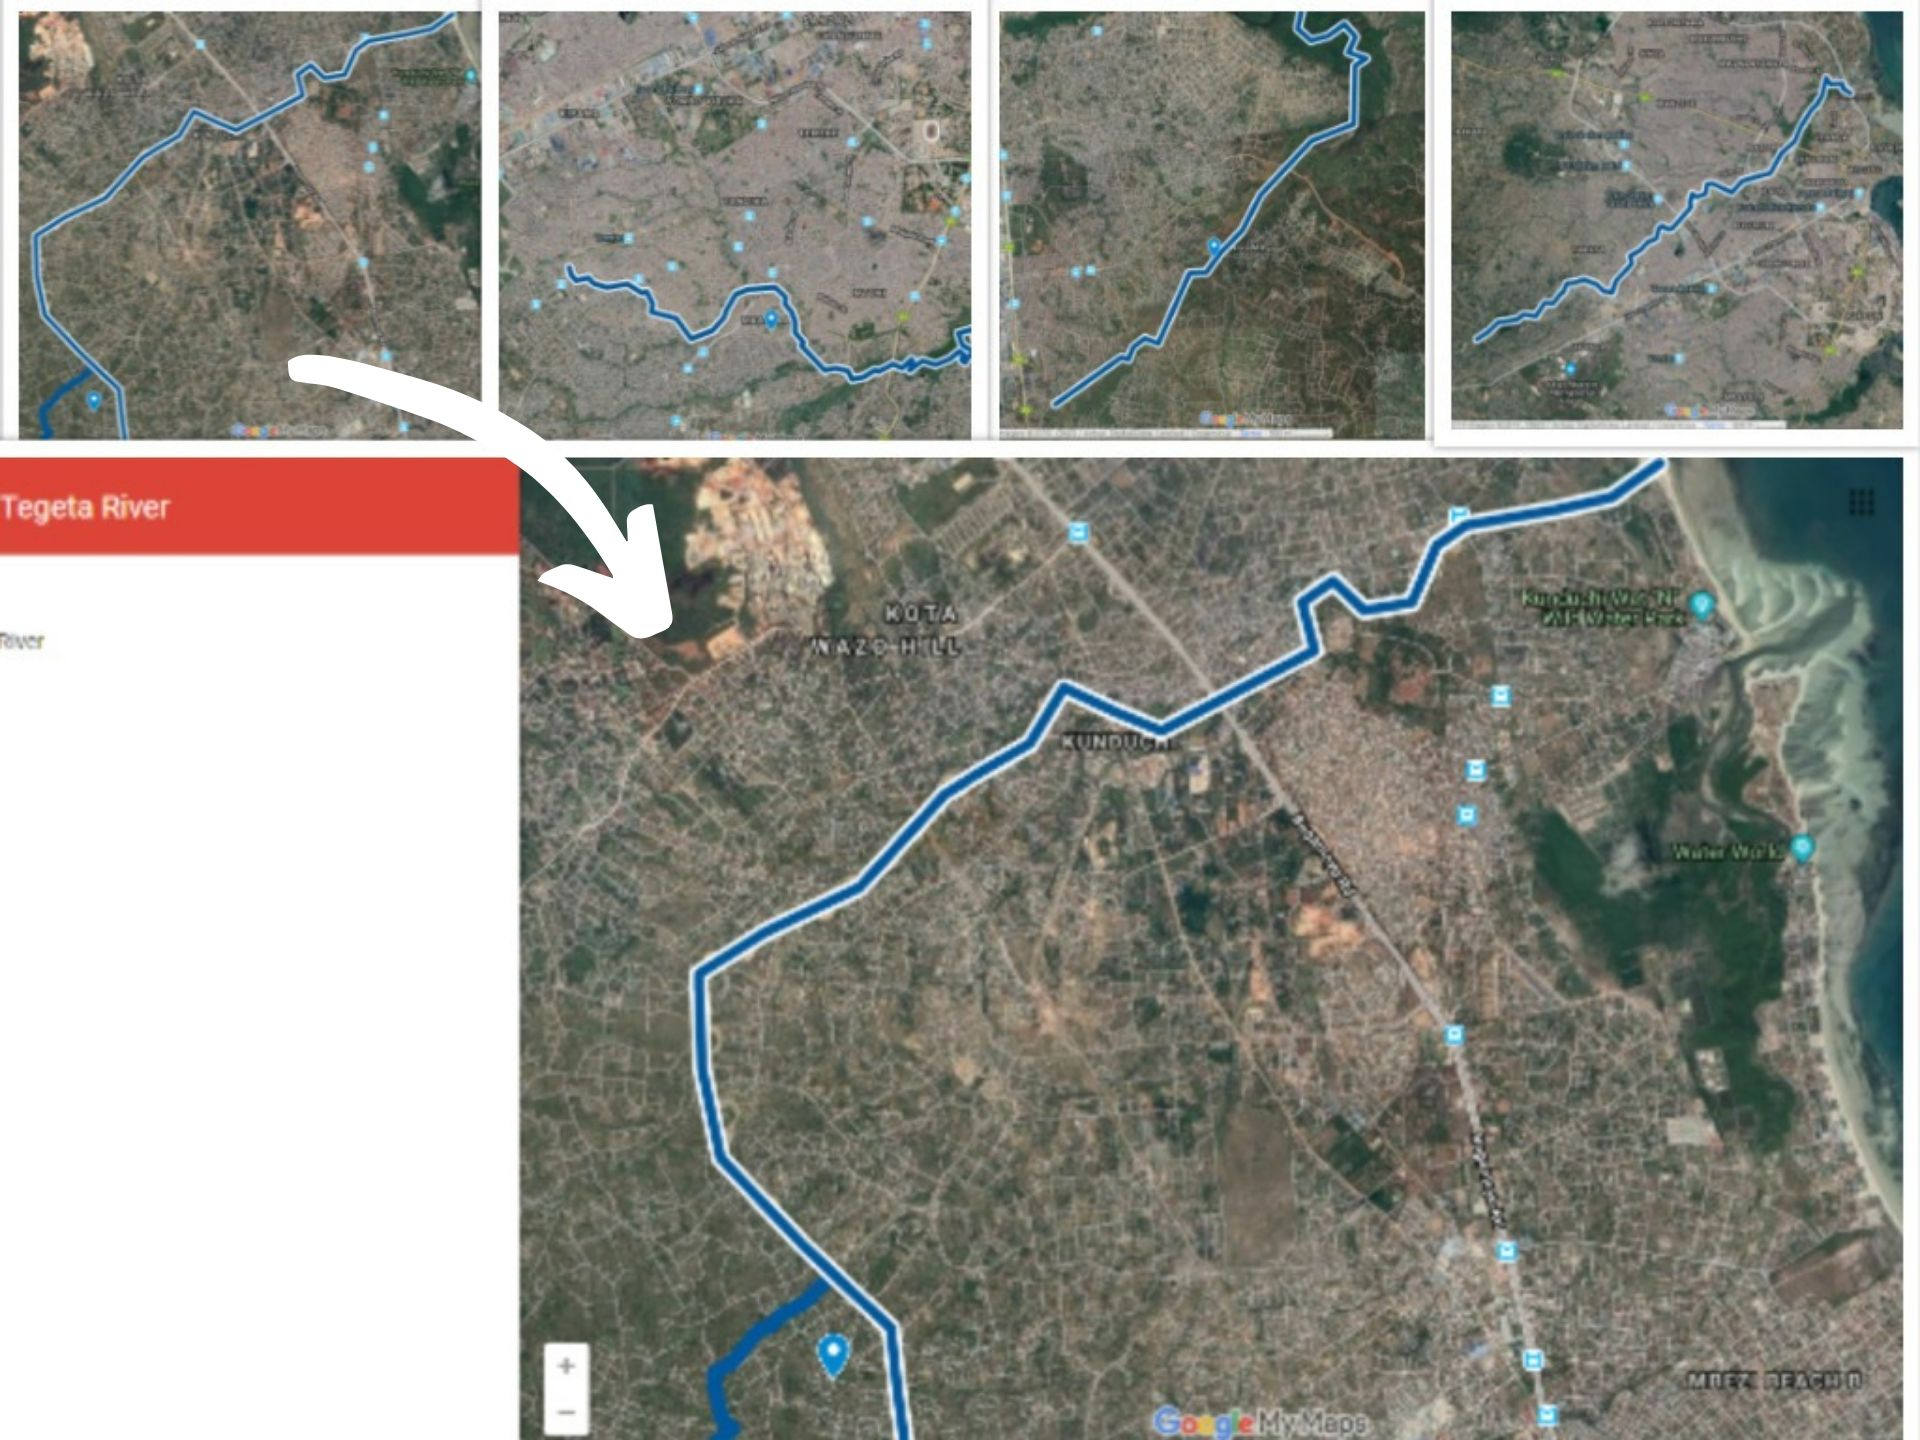
\includegraphics[width=0.8\textwidth]{images/image14.jpg}
    \caption{Screenshot showing missions plans of river mapping}
\end{figure}


\begin{multicols}{2}
\lipsum[0-5]
\end{multicols}

\section{Stakeholders}

\begin{multicols}{2}
\lipsum[0-5]
\end{multicols}

\subsection{Implementing Partners}

\begin{multicols}{2}
\lipsum[0-5]
\end{multicols}

\subsection{Beneficiaries}

\begin{multicols}{2}
\lipsum[0-5]
\end{multicols}

\subsection{Funders}

\begin{multicols}{2}
\lipsum[0-5]
\end{multicols}

\section{Methodology}

\begin{multicols}{2}
\lipsum[0-5]
\end{multicols}

\subsection{Drone Use}

\begin{multicols}{2}
\lipsum[0-5]
\end{multicols}

\subsection{Tools}

\begin{multicols}{2}
\lipsum[0-5]
\end{multicols}

\subsection{UHU Glue for Polystyrene Minor Repair}

\begin{multicols}{2}
\lipsum[0-5]
\end{multicols}

\subsection{MicroSD Cards for Swapping}

\begin{multicols}{2}
\lipsum[0-5]
\end{multicols}

\subsection{Reflector Vest}

\begin{multicols}{2}
\lipsum[0-5]
\end{multicols}

\subsection{Drone Processes}

\begin{multicols}{2}
\lipsum[0-5]
\end{multicols}

\section{Conclusion}

\begin{multicols}{2}
\lipsum[0-5]
\end{multicols}

\subsection{Achievements}

\begin{multicols}{2}
\lipsum[0-5]
\end{multicols}

\subsection{Challenges}

\begin{multicols}{2}
\lipsum[0-5]
\end{multicols}

\subsection{Lessons Learned}

\begin{multicols}{2}
\lipsum[0-5]
\end{multicols}
\subsection{Challenges}

\begin{multicols}{2}
\lipsum[0-5]
\end{multicols}

\section{Acknowledgements}

\begin{multicols}{2}
\lipsum[0-5]
\end{multicols}

\section{References}

\begin{multicols}{2}
\lipsum[0-5]
\end{multicols}

\subsection{Executive Summary}

\begin{multicols}{2}
\lipsum[0-5]
\end{multicols}

Objectives	16
\section{Acknowledgements}

\begin{multicols}{2}
\lipsum[0-5]
\end{multicolsTraining of Nipe Fagio Personnel	17
OpenDataKit (ODK) Collect Training	17
QGIS Training	18
Creation of Kobo Toolbox  server for data aggregation	18
Data Collection Tools	19
Map Literacy	19
Preparation of Building Clustering and Non-clustering Randomization Manuals	19
Waste management pilot in mapped areas with Nipe Fagio	20
Questionnaire	20
Data Cleaning using OpenRefine	21
Preparation of Web Interactive Map



\end{document}

\newpage  
